\documentclass[a4paper,12pt]{report}
\usepackage[T1]{fontenc} 
\usepackage[utf8]{inputenc}
\usepackage{subfig}
\usepackage{graphicx}
\graphicspath{ {./images/} }
\usepackage{epstopdf}
\usepackage{amsmath}
\usepackage{amsfonts}
\usepackage{amsthm}
\usepackage{array}
\usepackage{bm}
\usepackage{amssymb}
\usepackage{caption}
\usepackage{cite}
%\usepackage{subcaption}
\usepackage{epstopdf}
\usepackage{fancyhdr} 
\usepackage{fullpage}
\usepackage{eso-pic} 
\usepackage[english]{babel}
\usepackage{rotating}
\usepackage{tikz}
\usepackage{float}
\usepackage{rotfloat}
\usepackage[titletoc]{appendix}
\usepackage{booktabs}
\usepackage{multicol}
\usepackage{multirow}
\usepackage{lscape}
\usepackage{hyperref}
\usepackage{titlesec}
\usepackage{url}
\usepackage{colortbl}
	\definecolor{maroon}{rgb}{0.75, 0.75, 0.75}
\setlength\parindent{0pt}
\usepackage[export]{adjustbox}
\usepackage{wrapfig}
\usepackage{gensymb}
\usepackage[official]{eurosym}
\usepackage[nice]{units}
\usepackage{changepage}
\usepackage{pdfpages}
\usepackage{titlepic}
\usepackage{listings}
\usepackage{xcolor}
\usepackage{soul}
%\usepackage[prefix,intoc]{nomencl}
%\usepackage[nottoc]{tocbibind}
\RequirePackage{ifthen}
\usepackage{listings}
%\usepackage{tocloft}
\usepackage[framed,numbered]{matlab-prettifier}

\lstset{
  style      = Matlab-editor,
  basicstyle = \fontfamily{pcr}\selectfont\footnotesize, % if you want to use Courier
}

%\usepackage{ifpdf}
%\ifpdf
%  \usepackage{epstopdf}
%\fi

% Subtract 1 from counters that are used
\renewcommand{\thesection}{\thechapter.\number\numexpr\value{section}-1\relax}
\renewcommand{\thesubsection}{\thesection.\number\numexpr\value{subsection}-1\relax}
\renewcommand{\thesubsubsection}{\thesubsection.\number\numexpr\value{subsubsection}-1\relax}
\setcounter{secnumdepth}{3}

\setcounter{chapter}{0}% Not using chapters, but they're used in the counters
    
\title{Review chapter}
\author{Gabriela Pardo Arteaga 4617630}

\date{\today}
\begin{document}
\maketitle


%Say very briefly 1) what the review is about, 2) what the main content is, 3) what the main aim or objectives are, and 4) what the main findings are. End with a strong sentence that highlights the significance of the work presented in the review and any envisioned long-standing contribution to the body of knowledge.



%%%Summary
\section*{Abstract}
%Say very briefly 1) what the review is about, 2) what the main content is, 3) what the main aim or objectives are, and 4) what the main findings are. End with a strong sentence that highlights the significance of the work presented in the review and any envisioned long-standing contribution to the body of knowledge.
Olympic sailing is characterize by one-boat design in each class, with its particular rules. %These classes are: one windsurfing board, two keelboats and four variants on the dinghy.
Because improvements on the boat are not allow; the scope for many researches is focus on the athlete, enhancing strength and other motor skills. On each class, the competition stand for many races and days where the configurations of the route and the environmental conditions diverse from each other. The winner is the one with the lowest score. In each race, points are given  and %fand in each race every position gives points; 
the higher position the lower score. Athletes and coaches confront distinctive scenarios for which they take different decisions in order to win. One of these decisions refers to the sailing direction taken at the start line.

During competition, it is the athlete who decide the number maneuvers and the direction of each; specially on the upwind condition, the boat sails against the wind
%Since the sailboat can not displace towards the wind, tacking manoeuvers are perform. This type of path is described as 
in a zig-zag pattern that can be started on the left- or on the right-hand side. %Another condition is dictated when the boat is dis- placed in the same direction as wind. These conditions shows that feasible paths are asymmetrical[Dol12]. 
Because athletes are not allow to get any information or feedback from coaches; the information of how to course the race before competition is crucial. \newline
%As in many race competitions, the winner is the one that first cross the end line. In other words
The fastest path results from a trajectory sailed with a minimal time, independently of its length. Because trajectories are defined by the route to sail, the wind and current fields characteristics as intensity and direction, and the sail angle respect to the wind. The selection of the fastest path requires the discretization of the area cover by the route. If wind and current fields are not constants, they also required the discretization respect to location and time. These process define the granularity of the problem to solve and in consequence the computation time to find a solution. % The area of sail  These two discretizations are  Because of this, the problem can be define as an optimization problem with the objective to miminizes the time of the trajectory to f 
%to with the minimal time, The relevance of the fastest path is because during competition the boat that first cross the end line is the winner which means

The purpose of this study is to model the path for sailing competitions and optimize the minimal time of sailing routes for the Laser (Olympic class) shaped by wind. Furthermore, identify the effects of different time steps on the resulting times and trajectories.
%In other words,%the critical variables influenced by the wind that determine it.
%the study seek 
%To answer the question, What is the optimal sailing route for the Laser (Olympic class) shaped by wind. The objective is to analyze the sensibility of the optimal route due to changes on the wind field and start times. This will determine the zones and the shape trajectory of the optimal path. 
%and conditions that shape not only the optimal but the least route also. 
To answer this question first, the physical model of yachts was reviewed. Despite the similarities between dinghies(Laser boats) and yachts, the physical model was adapted by adding two coefficients related with sails which indicate%the research focusing on dinghies is significantly lower as consequence adaptations have been made to represent
how different is steering a dinghy from a yacht. Moreover, these adaptations are reflected on the %These adaptations are related with the
Velocity Prediction Polar (VPP)diagram. By using the VPP and the wind intensity is possible to set the direction at which the dinghy reach is maximum velocity respect to the wind. This approach is known as Velocity Made Good (VMG).%  and to more specific and the use of sails
%Despite the similarities between dinghies and yachts, the research focusing on dinghies is significantly lower as consequence adaptations have been made to represent how it is steering, one of this is related with the VPP's and the use of sails. The same situation happens when the topic of research is related with optimal routes.  Since Olympic sailing is focused on the seamanship, the understanding of physical principals intends to provide or reveal hints that helps them to train and contest effectively regardless the location and routes. \newline

%The report answers the question of what device should be developed 
%%most be included on a portable device% 
%for people without impaired limbs; such as the ageing,  to enhance the motion of the upper limb in terms of force and what are the most (technically) feasible features to include on it to improve the life quality of the users.% %design that enhances the human force of the upper limb. 
%To answers these questions first  
%%This will be done by means of the 
%a literature study about the topic was done. Then, an inventory analysis was developed about the devices available on the market that enhance force. From this analysis,  the requirements and the critical features were identified and three concepts were developed. %the .% 
%This report asses them 
%%these portable designs %the three concepts  
%with the multi-criteria analysis method to identify the most feasible design to enhance the force of the upper limb for people without impaired limbs. The design %with the higher score 
%obtained from the assessment was the powered exoskeleton with monitoring system.
The algorithm developed is limited to dinghies which is one of the Olympic boat classes and the smallest; and it was validated by comparing its results against the results of previous races located at Hyères, France during 2018. Three wind conditions were tested, first is was assume that the wind intensity and direction are constant along the area of the route; the second, considers a forecast wind field as time-space-dependent variable changing every 10 minutes without current and neglecting the wave disturbances and twisting effects on the sail, the last test condition uses the wind measurements took during the competition. 

The preliminary tests show that results are closer when the wind is assuming constant and when VPP used is estimating from the top 10 competitors of the competition. The dynamic model of the dinghy requires further research to give more predictable and accurate results. Olympic Classes as dinghy is not a widespread research topic. Besides most of the findings related to path optimization for boats are related with cargo ships and vessels, where the main objective is to minimize the fuel costs, because these ship can be set to navigate at a constant speed. The influence of the wind is not the same as for the Olympic Classes. Another consideration that should be taken is related with the movement of the sailor which affect the equilibrium of the boat and therefore the maximum speed that could be reach.  %The reason for this is that limited data was available, as sailboat modelling is not a widespread
 %Also, on formulating a sailing trajectory optimization as an optimal control problem, very limited information was available.
%Although quite some problems have been solved, the results can be improved by future re- search, by addressing the most important recommendations below.
%Towing tank, open water and wind tunnel tests could be carried out to determine the hy- drodynamic and aerodynamic characteristics of the dinghies, to be able to incorporate higher order dynamics into the model over a wider range of boat and wind speeds.
%In this thesis the focus was on determining the advantage in an upwind leg of the route based on currents, but a more detailed model could also help in the future to optimize and analyse the trimming of the sail, rudder action or even the movement of the sailor.
%Furthermore, the focus was on the influence of currents, but in the results some cases subject to wind variations were treated. In future research wind dynamics could be implemented much more detailed. For this, a proper wind model should be developed. But this would need specific attention because wind is much more subject to uncertainties than currents.
%Furthermore, other boat types, multiple competitors and weather uncertainties could be im- plemented in future research.

The report is set as follows: Chapter 1 refers to the basics concepts of sailboat and wind fields, Chapter 2 describes the mathematical model for sailboat in general and the modifications required. The validation of the model is reviewed on chapter 3. In Chapter 4 the obtained results are analyzed and finally the conclusions and recommendations are described in Chapter 5.\par 
\tableofcontents
%\gobbletocpage
\addcontentsline{toc}{section}{Abstract}
\newpage
\chapter{Introduction}

%Introduce the general area of interest that the contents of the review deal with, setting out any advancements and challenges of interest. Then introduce more fully the specific topic addressed in the review and you can then to go on to state any main aim or objectives to be met. Say very briefly what is to come in the layout of the review. Note: the Introduction should include general references to back up the points made.
% Establishing the field
%Definition:
%What are the Olympic classes sailing?
%How are the competitions setting  up?
%What does position and direction means?
%What time steps are you referring for the wind forecast, which sizes?

In recent years the integration of new technologies on training programs of professional athlete have been increased. Not only to enhance their motor skills, and to prevent injuries but also to obtain better results with a minimal time and in a more efficient process. For example, the use of information that specify the conditions or parameters that delivers the best results to win have gained more popularity within the sport community. The involvement of science like kinesiology \cite{sjogaard2015science}, movement science; and engineering is not only concentrated in the athletes furthermore in the elements and factors that can not be controlled by them but by those which impact their results. One of these sports is sailing where athletes have to guide the boat under different weather conditions and where time is critical to win the race.\par
During sailing races such as coastal, inland waterways and lakes athletes are not allowed to get any information from coaches during the race; for this reason, their preparation and training is not only physical. During training they acquire skills to anticipate the weather changes and at the same time maneuvers to improve the performance of the boat. \par
%For example, a well know competition and classes are the Olympic sailing competitions which take place on coastal and improvements on the boat are not allow. \\
In this section, the research problem, its relevance and the objectives are going to be presented. For this, a brief definition of Olympic sailing classes and courses are going to be explained followed by an explanation of the information considered by the coaches and athletes to plan the strategy before the competition takes place which most of the time refers to the weather forecast. These data provide a framework to set-up the assumptions and limitations considered in this research. \par 
\section {Olympic Sailing} \label{sec:olympic classes}
The Olympic Sailing Classes are characterized by the rule of one-design boat. The intention of this is to leave out the influence of technology on the results and focus on the abilities of the athlete to perform effectively; for this reason, the scope for many researches is on the athlete only. The figure \ref{fig:olymp_cla} shows the names and categories of the current classes that the International Federation of sailing defines as Olympic Classes. The list is subject to change and it is reviewed every 4 years when the Olympic Games have been completed.\par 
The dinghy is not only the smallest boat propelled by wind, but the one with more classes. The differences between their classes relies on the dimensions of the boat and sail. These dimensions are determine by the number of crew members,1 or 2, and their gender. This is one of the reasons why this research is going to use the dinghy as a reference boat, another reason is due to its similarity physically and mathematically with yachts which has been studied since 1979 \cite{marchajaereo1979}. \par 

\begin{figure}[ht]
\centering
 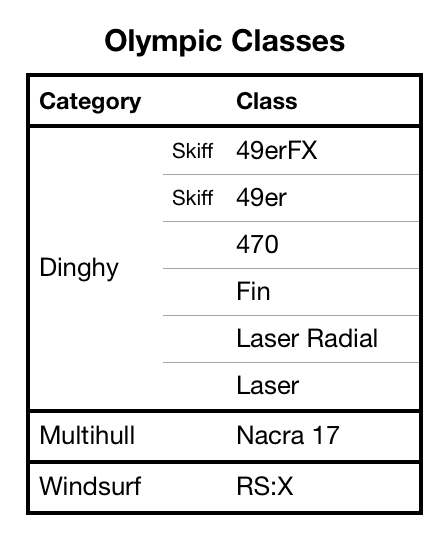
\includegraphics[width=0.32\textwidth]{olym_classes.png}
  \caption{Olympic classes \cite{sailoly}.}
\label{fig:olymp_cla} 
\end{figure}

The competition in each class stand for many races and days where the configurations of the course vary according the environmental conditions. In each race, points are given according is arrival position; the faster, the lower score. The winner is the one with the lowest score. Under this competing format athletes and coaches confront distinct scenarios for which they take different decisions at the start line. One of these decisions refers to the initial sailing direction. The importance of it is related to the configuration of the course.\par 

\section{Competition Course}\label{tracks}
The most common form of a sailing competition is the fleet racing where all participants race around a course and start at the same time along a line. Here, not only the reaction time is important, but the direction that allow the maximum speed that could be attained. Usually two different types of courses took place in the Olympic classes. Figure \ref{fig:trap_c} shows the singular trapezoid course which is defined by a separate start and finish line and 4 points around (buoys); these 6 elements define the legs of the competition and the first leg is usually the longest one and it is running against the wind.
The trapezoid course is the most completed format courses, the other formats are a partial representation of it, considering only some legs which are already represented in the trapezoid course.\par 
%The other course is the windward/leeward, figure \ref{fig:wl_c} this is simply a two-leg race orientated in such way that the first leg is sail against the wind (called a beat) and the second leg is sail with the wind (called a run). If boats are sailing neither with nor against the wind, the leg is called reach. 

The courses characteristics and conditions of race, these are subject to change every 4 years also and they are regulated in the next way \cite{race_pol}: The length and angles of each leg are defined in such way that the course could be completed in maximum 1 hour and the trapezoidal course can be contained in a grid size of 2km by 2km.  Another consideration is the area of the course,  which most of the time is expressed in nautical miles (nm). Figure \ref{fig:olymp_areas_rio} is an example of how the sailing areas are defined by a circular area, within this circle the trapezoid should be located. \par 
Furthermore, the wind conditions refer to the average wind speed in addition to its shift direction. The race will not start if the average wind speed is less than 4 knots(kn)[2 m/s] or more than 25 knots(12.86 m/s) over the entire course. %However, the maximum wind shift allowed is 10\deg. 
If wind conditions are not meet the race could be delayed, and if the race has already started, it is possible a change in the course or an abandon of the race \cite{race_pol}. With this, it is clear how important is the wind for sailing; however to understand how it interacts with the boat and the athlete first it is required to know the physics of sailing. \par 

\begin{figure}[ht]
\centering
 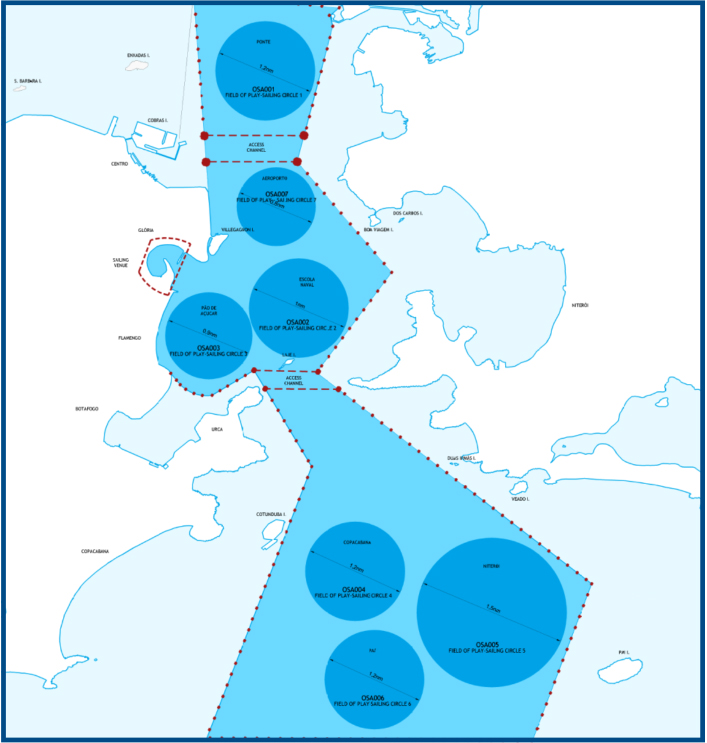
\includegraphics[width=0.6\textwidth]{16_OG_RaceAreasNOR.jpg}
  \caption{Sailing Races Areas. Olympic Games Rio 2016 \cite{instr_rio}.}
\label{fig:olymp_areas_rio} 
\end{figure}

\begin{figure}[ht]
  \centering
  \subfloat[Trapezoid Course ] {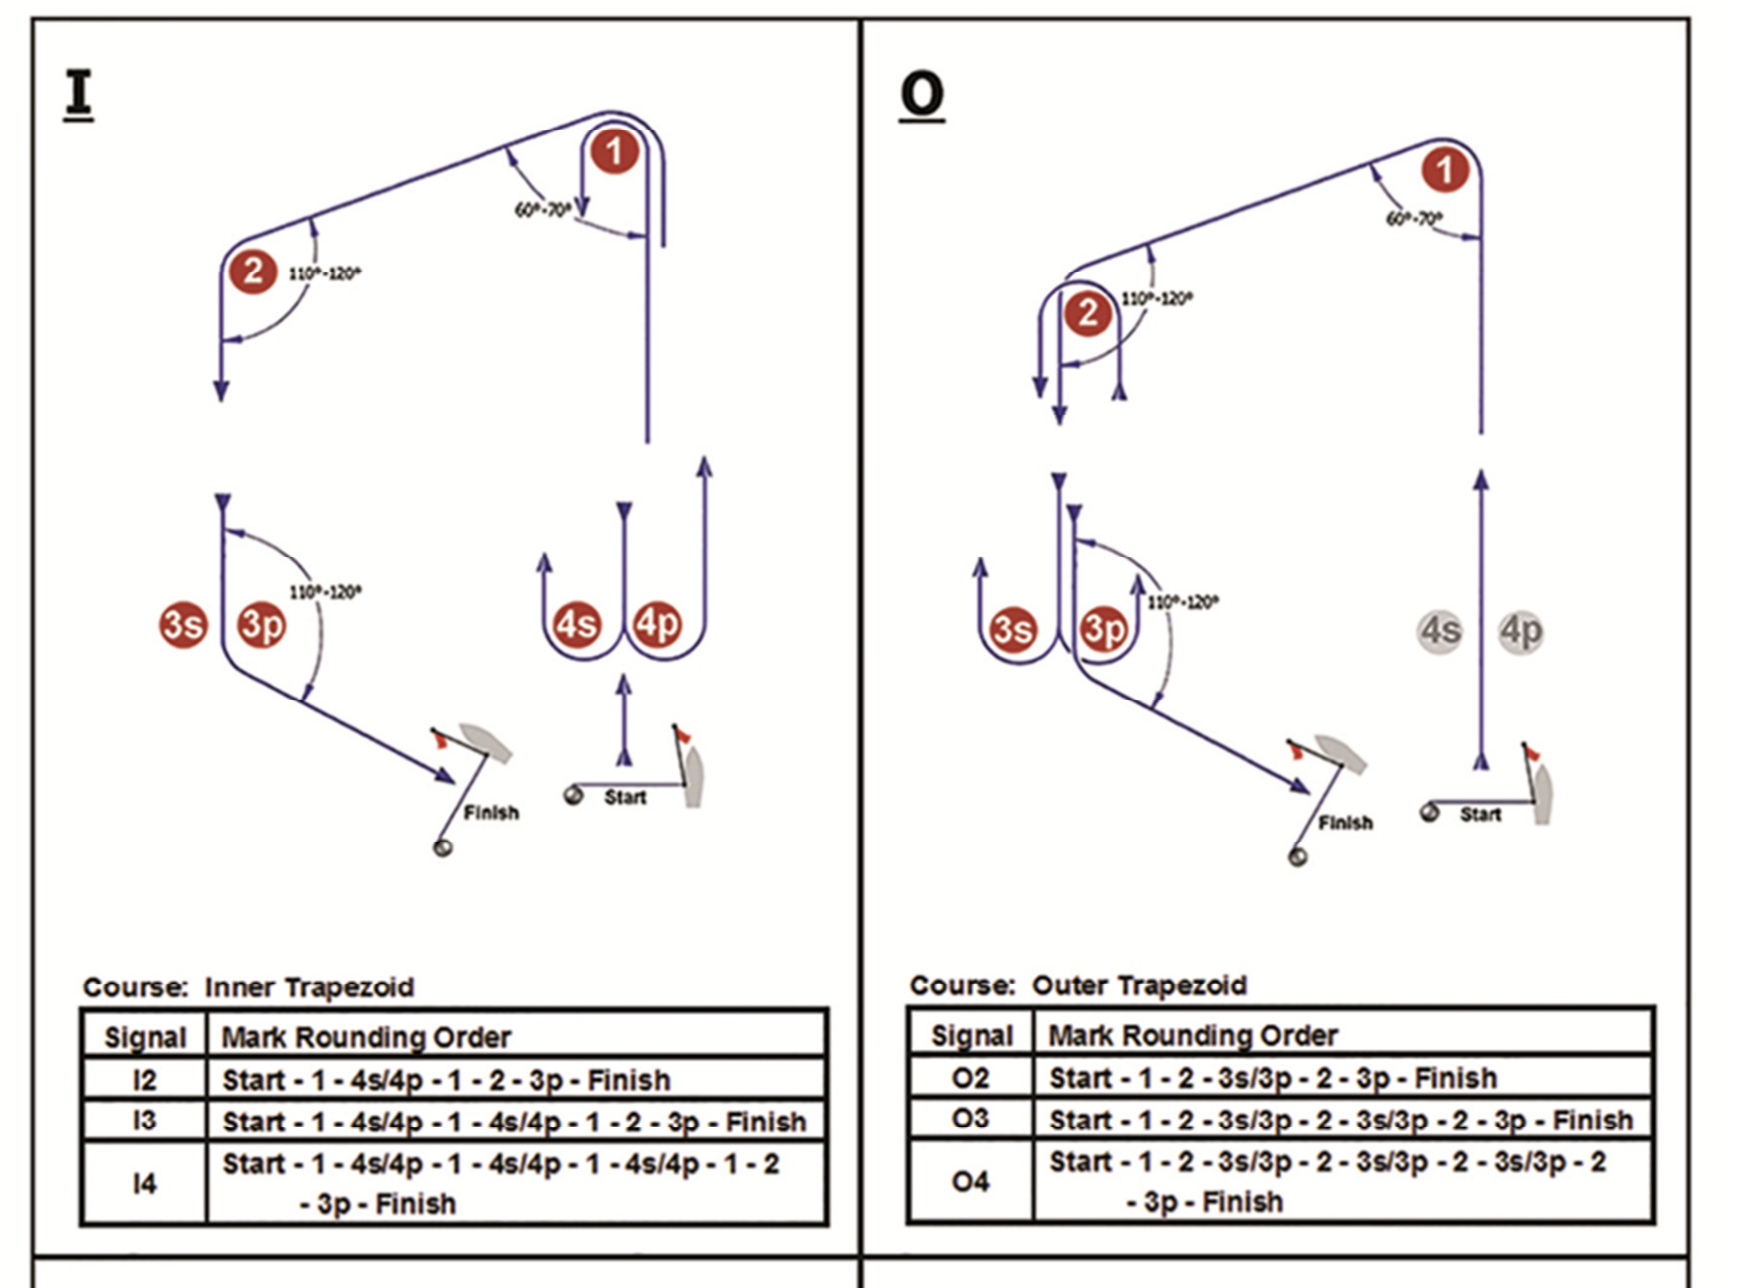
\includegraphics[width=0.53\textwidth]{trap_course.png}\label{fig:trap_c}}
  \hfill
  \subfloat[Windward / leeward course] {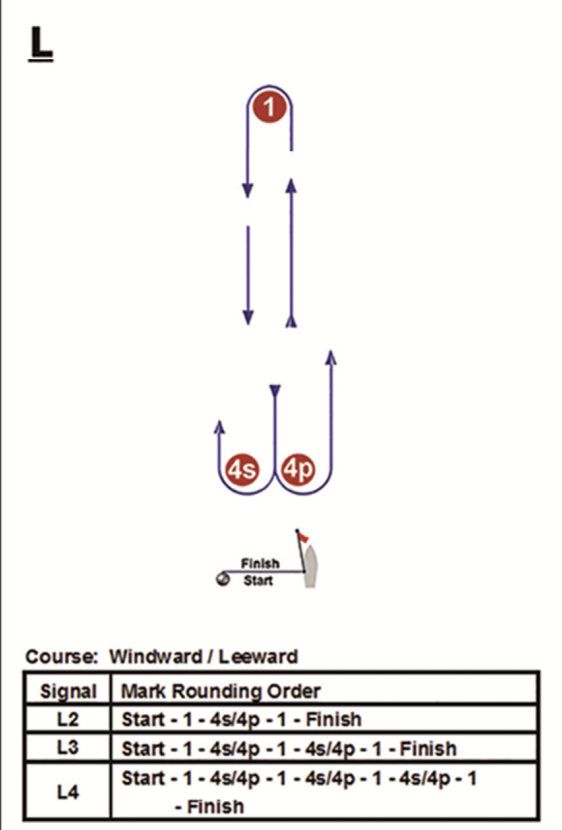
\includegraphics[width=0.25\textwidth]{l_w.png} \label{fig:wl_c}}
  \caption{Types of courses \cite{instr_rio}.}
\label{fig:typecourses} 
\end{figure}

The direction of the boat respect to the wind determines the type of maneuvers and trajectory that most be followed. For example the first leg of the trapezoid course runs against the wind and boats can not displace towards it. The maneuvers used in this condition is shown in figure \ref{fig:tacking}, the trajectory forms a zig-zag patterns that can be started on the left- or on the right-hand side and each change on the heading direction is known as tack. \par 

Even when the trajectory looks symmetrical it is important to remember that the wind is not constant all the time. During the competition, it is only allow to have maximum shift of 10 \degree \cite{race_pol}. So far there is no evidence to accept or reject this symmetric condition. This raises the question what direction should be taken when the boat has to run against the wind, in other words what is the path with the minimal time to follow?. To answer this question athletes and coaches rely on their previous knowledge and experience to decide what is the starting direction. This previous knowledge is based on geographical characteristics around the area of the course and exposure to the site. Top athletes for the Olympic Games train in the site at least one year before the event.\par 
\begin{figure}[ht]
  \centering
  \subfloat[Tacking Maneuver \cite{denny2009float}.] {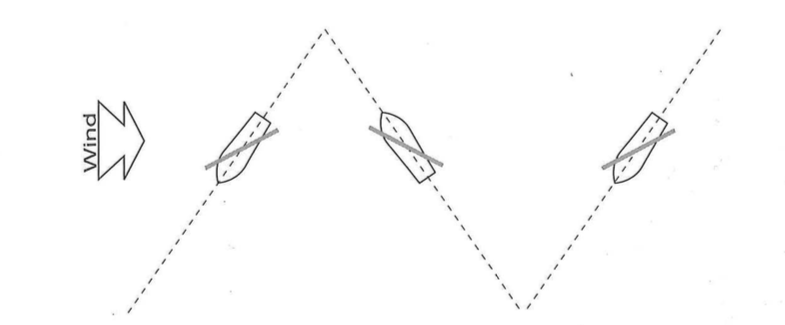
\includegraphics[width=0.45\textwidth]{tacking.png}\label{fig:tacking}}
  \hfill
   \centering
  \subfloat[Tacking maneuver]{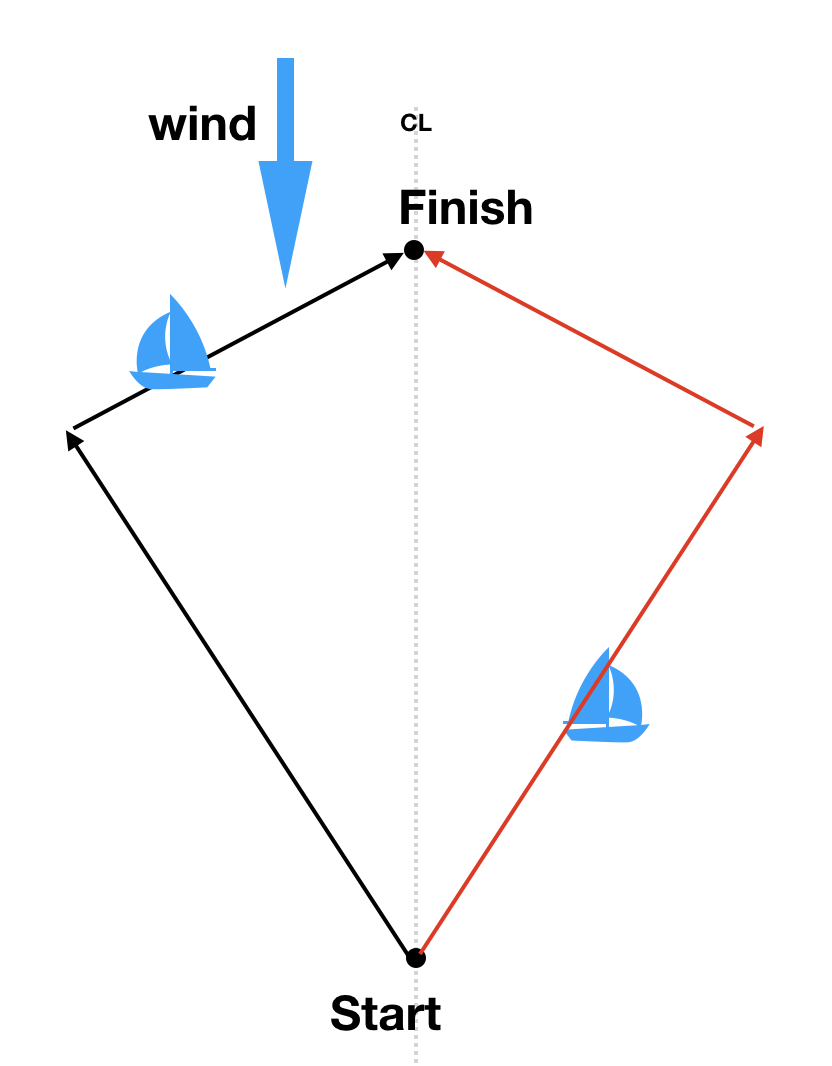
\includegraphics[width=0.35\textwidth]{images/upwind_sym.png}\label{tack_jib}}
  \caption{Tacking maneuver against the wind.}
\label{fig:tack_against_wind} 
\end{figure}

\section{Weather Forecast}
Weather forecast is calculated by super computers and updated every certain time according regions, usually every three hours. Due to its complexity different agencies and governments have developed models to predict the weather in global terms, so local predictions can be made. This local predictions take into account the global model and adjusted according local measurements allowing to being update every hour with a grid resolution of 3km by 3km \cite{warner2010numerical}. \par

Uncertainty weather is a typical condition that yacht competitions and maritime transportation have to manage. In the case of yacht competitions courses could take days, weeks or even months; like the \textit{Volvo Ocean Race}, which is an around the word. The path planning for this kind of boats has been researched specially by maritime and logistics sciences a less number of publications can be found for yacht races and autonomous vehicles, and just a few number of researches refer to Olympic races. \par  

 Because, Olympic races have a duration of maximum one hour inside a grid of size 2km by 2km and local forecast is updated every hour within a grid of 3km by 3km. The information that coaches and athletes can access previous the race do not match the characteristics and needs for them at first instance.\par 
 
 Short course and long courses races are different. Short courses, for example, are more sensitive to random fluctuations \cite{philpott2001optimising}. Furthermore, the direction to take at the beginning of the competition could be the optimal just for a couple of minutes but not for the whole race. Time on Olympic sailing classes is critical to win; but at the same time a higher resolution on time and space for the weather is more costly in terms of computation effort for weather and the minimal time trajectory processing. The impact of a fine resolution vs a coarse on the time trajectories is unknown in the other hand, it is also unknown how small this resolution should be in order to be significant for the  race.\par 
 
 \section{Aim of the Research}
 
This research proposes an algorithm to model sailing trajectories shaped by wind for Olympic Classes which %more specific for Laser (dinghies) competitions %and optimize it to obtain the minimal time for the Laser (Olympic class). 
can answer the question, What is the optimal sailing route shaped by wind for the Laser (Olympic class)?  The study suggest that the sensibility of the optimal route due to changes on the wind field and start direction can define zones and shape the trajectory for minimal time paths. \par 

Furthermore, it demonstrates the effects of 3 different time steps and spacial resolutions on the resulting trajectories with its times. This will be done by means of experiments using the optimization of the algorithm proposed. The results(simulations) obtained can be compared against the measurement data of the selected race. In this way, it is possible to identify the size of the differences. and quantify the effect of the uncertain weather over the trajectory and times.\par 
%In other words,%the critical variables influenced by the wind that determine it.
%the study seek 
%To answer the question, What is the optimal sailing route for the Laser (Olympic class) shaped by wind. The objective is to analyze the sensibility of the optimal route due to changes on the wind field and start times. This will determine the zones and the shape trajectory of the optimal path. 
%and conditions that shape not only the optimal but the least route also. 
%To answer this question first, the physical model of yachts was reviewed. Despite the similarities between dinghies(Laser boats) and yachts, the physical model was adapted by adding two coefficients related with sails which indicate%the research focusing on dinghies is significantly lower as consequence adaptations have been made to represent
%how different is steering a dinghy from a yacht. Moreover, these adaptations are reflected on the %These adaptations are related with the
%Velocity Prediction Polar (VPP)diagram. By using the VPP and the wind intensity is possible to set the direction at which the dinghy reach is maximum velocity respect to the wind. This approach is known as Velocity Made Good (VMG).%  and to more specific and the use of sails
%Despite the similarities between dinghies and yachts, the research focusing on dinghies is significantly lower as consequence adaptations have been made to represent how it is steering, one of this is related with the VPP's and the use of sails. The same situation happens when the topic of research is related with optimal routes.  Since Olympic sailing is focused on the seamanship, the understanding of physical principals intends to provide or reveal hints that helps them to train and contest effectively regardless the location and routes. \newline

 \section{Terms, conditions and limitations}
 %This report asses them 
%%these portable designs %the three concepts  
%with the multi-criteria analysis method to identify the most feasible design to enhance the force of the upper limb for people without impaired limbs. The design %with the higher score 
%obtained from the assessment was the powered exoskeleton with monitoring system.
The algorithm developed is limited to dinghies, the smallest and one of the most used boats on the Olympic classes. More specific, the Laser Class with motion over the XY plane.  The 2D model proposed was validated by comparing the results of the simulations obtained against the results Laser races located at Hyères, France during 2018. The three wind conditions tested are: first, a constant wind intensity and direction along the area of the route; the second, considers a forecast wind field as time-space-dependent variable changing every 10 minutes over 1 km by 1km grid size without current and neglecting the wave disturbances and twisting effects on the sail, the last test condition uses the wind measurements took at 20 Hz during the competition. \par 

Olympic Classes like dinghy is not a widespread research topic. Besides most of the findings related to path optimization for boats are related with cargo ships and vessels, where the main objective is to minimize the fuel costs, because these ship can be set to navigate at a constant speed. The influence of the wind is not the same as for the Olympic Classes. The movement of the sailor was not considered as a variable since it was assume that the athlete is skill enough to keep the equilibrium of the boat and  maximize speed without further complications. In the case of the crew weight, the simulations used the weight proposed by \cite{laser_opt}, which is between	55 and 70 kg.\par 

 
 \section{Report Structure}
The report is set as follows: chapter 2 refers to the basics of sailboat; the forces and equation that governs its motion in general and the modifications required for the purposes of this research. The validation of the model and how the wind model is integrated is reviewed chapter 3. In chapter 4,the optimizer algorithm is explained and how the model is implemented;  the obtained results are analyzed in chapter 5 and finally the conclusions and recommendations are described in chapter 6.\par 

%has been considering in the development of methods for the optimal path.
%The random fluctuation over the time is more sensitive on short courses rather long coursed.
%Taking good decisions on time depends on: the available data and processing time. The processing time refers to the time it takes to converted the available data into meaningful information. These two variables have been approaching by Different researchers to obtain 




%Because of this Philpott \cite{philpott2001optimising} describe a method for each condition to figure out the optimal path.  The weather variables in a short courses were considered to have a minimum spatial variation, although they enclose a random component due to its dependence over time.\\


%With this method the area and time have to being discretize, more over the it consider different states or possibles angles at which the wind will be directed. Which means that each location has to evaluate each of the states and find the optimal path among  \textit{n} stages.  The larger or the smaller the the discretization the more locations to solve according each stage, which seem that the computational effort will grow considerably since each leg has to be evaluated.  The paper does not mention the computational effort nor the difference of time that can be achieve by using it.Philpott \cite{philpott2001optimising}



\bibliographystyle{unsrt} %ieeetr %alpha %apalike
\bibliography{sections/thesisref}

\end{document}